% options:
% thesis=B bachelor's thesis
% thesis=M master's thesis
% czech thesis in Czech language
% slovak thesis in Slovak language
% english thesis in English language
% hidelinks remove colour boxes around hyperlinks

\documentclass[thesis=B,czech]{FITthesis}[2012/06/26]

\usepackage[utf8]{inputenc} % LaTeX source encoded as UTF-8

\usepackage{graphicx} % graphics files inclusion
\usepackage{amsmath} % advanced maths
\usepackage{amssymb} % additional math symbols

\usepackage{dirtree} % directory tree visualisation

% % list of acronyms
\usepackage[acronym,nonumberlist,toc,numberedsection=autolabel]{glossaries}
\iflanguage{czech}{\renewcommand*{\acronymname}{Seznam pou{\v z}it{\' y}ch zkratek}}{}
\makeglossaries

\newcommand{\tg}{\mathop{\mathrm{tg}}} %cesky tangens
\newcommand{\cotg}{\mathop{\mathrm{cotg}}} %cesky cotangens

% % % % % % % % % % % % % % % % % % % % % % % % % % % % % % 
% ODTUD DAL VSE ZMENTE
% % % % % % % % % % % % % % % % % % % % % % % % % % % % % % 

%%%%%%%%%%%%%%%%%%%%%%%%%%%%%%%%%%%%%%%%%%%%%%%%%%%%%%%%%%%% <nesrotom>

\usepackage{float}

\usepackage{algorithm}% http://ctan.org/pkg/algorithms
\usepackage{algpseudocode}% http://ctan.org/pkg/algorithmicx
\usepackage{pseudocode}

\let\mylistof\listof
\renewcommand\listof[2]{%
\mylistof{algorithm}{Seznam algoritmů}%
}

%\mylistof{algorithm}{}

%%%%%%%%%%%%%%%%%%%%%%%%%%%%%%%%%%%%%%%%%%%%%%%%%%%%%%%%%%%% </nesrotom>

\department{Katedra \ldots (DOPLŇTE)}
\title{Doplňte název práce}
\authorGN{Doplňte Vaše křestní jméno/jména} %(křestní) jméno (jména) autora
\authorFN{Doplňte Vaše příjmení} %příjmení autora
\authorWithDegrees{Doplňte Vaše jméno a tituly} %jméno autora včetně současných akademických titulů
\supervisor{Doplňte jméno vedoucího práce}
\acknowledgements{Doplňte, máte-li komu a za co děkovat. V~opačném případě úplně odstraňte tento příkaz.}
\abstractCS{V~několika větách shrňte obsah a přínos této práce v~češtině. Po přečtení abstraktu by se čtenář měl mít čtenář dost informací pro rozhodnutí, zda chce Vaši práci číst.}
\abstractEN{Sem doplňte ekvivalent abstraktu Vaší práce v~angličtině.}
\placeForDeclarationOfAuthenticity{V~Praze}
\declarationOfAuthenticityOption{4} %volba Prohlášení (číslo 1-6)
\keywordsCS{Nahraďte seznamem klíčových slov v češtině oddělených čárkou.}
\keywordsEN{Nahraďte seznamem klíčových slov v angličtině oddělených čárkou.}

\begin{document}

% \newacronym{CVUT}{{\v C}VUT}{{\v C}esk{\' e} vysok{\' e} u{\v c}en{\' i} technick{\' e} v Praze}
% \newacronym{FIT}{FIT}{Fakulta informa{\v c}n{\' i}ch technologi{\' i}}

\begin{introduction}
	%sem napište úvod Vaší práce
\end{introduction}

%%%%%%%%%%%%%%%%%%%%%%%%%%%%%%%%%%%%%%%%%%%%%%%%%%%%%%%%%%%%%%%%%%%%%%%%%%%%%%
%%%%%%%%%%%%%%%%%%%%%%%%%%%%%%%%%%%%%%%%%%%%%%%%%%%%%%%%%%%%%%%%%%%%%%%%%%%%%%
%%%%%%%%%%%%%%%%%%%%%%%%%%%%%%%%%%%%%%%%%%%%%%%%%%%%%%%%%%%%%%%%%%%%%%%%%%%%%%
%%%%%%%%%%%%%%%%%%%%%%%%%%%%%%%%%%%%%%%%%%%%%%%%%%%%%%%%%%%%%%%%%%%%%%%%%%%%%%
%%%%%%%%%%%%%%%%%%%%%%%%%%%%%%%%%%%%%%%%%%%%%%%%%%%%%%%%%%%%%%%%%%%%%%%%%%%%%%
%%%%%%%%%%%%%%%%%%%%%%%%%%%%%%%%%%%%%%%%%%%%%%%%%%%%%%%%%%%%%%%%%%%%%%%% begin
%%%%%%%%%%%%%%%%%%%%%%%%%%%%%%%%%%%%%%%%%%%%%%%%%%%%%%%%%%%%%%%%%%%%%%%%%%%%%%
%%%%%%%%%%%%%%%%%%%%%%%%%%%%%%%%%%%%%%%%%%%%%%%%%%%%%%%%%%%%%%%%%%%%%%%%%%%%%%
%%%%%%%%%%%%%%%%%%%%%%%%%%%%%%%%%%%%%%%%%%%%%%%%%%%%%%%%%%%%%%%%%%%%%%%%%%%%%%
%%%%%%%%%%%%%%%%%%%%%%%%%%%%%%%%%%%%%%%%%%%%%%%%%%%%%%%%%%%%%%%%%%%%%%%%%%%%%%
%%%%%%%%%%%%%%%%%%%%%%%%%%%%%%%%%%%%%%%%%%%%%%%%%%%%%%%%%%%%%%%%%%%%%%%%%%%%%%

\chapter{Úvod do problematiky}

\section{Použití násobení matic}

TODO: kde se pouziva nasobeni matic

\section{Matice}

Matice \textbf{A} typu ($m$, $n$) je $m n$ uspořádaných prkvů z množiny $\mathbf{R}$. O prvku $a_{r,s} \in \mathbf{R}, r \in \{1,2,\hdots,m\},s \in \{1,2,\hdots,n\}$ říkáme, že je na r-tém řádku a~s-tém sloupci matice \textbf{A}. Matici \textbf{A} zapisujeme do řádků a~sloupců takto:
\begin{align}
\mathbf{A}=\begin{pmatrix}
a_{1,1} & a_{1,2} & \cdots & a_{1,n} \\
a_{2,1} & a_{2,2} & \cdots & a_{2,n} \\
\vdots  & \vdots  & \ddots & \vdots  \\
a_{m,1} & a_{m,2} & \cdots & a_{m,n}
\end{pmatrix}
\end{align}

Matici \textbf{M} typu ($m$, $n$), kde všechny její prvky jsou rovny nule, nazýváme \textit{nulovou maticí.}

O~matici typu ($m$, $n$) budeme říkat, že je $m$~široká a~$n$~vysoká. Pokud o~matici řekneme že má velikost $n$, myslíme tím, že je typu ($n$, $n$).

\section{Vektor}

Matici \textbf{V} typu (1, n) nazveme vektorem.

TODO=popsat vektory poradne
FIXME=muzu to takhle zjednodusit?

\section{Násobení matic}

Buď \textbf{A} matice typu ($m$,$n$) s prvky $a_{i,j}$ a \textbf{B} matice typu ($n$,$p$) s prvky $b_{j,k}$. Definujeme součin matic $\mathbf{A} \cdot \mathbf{B}$ jako matici \textbf{C} typu ($m$,$p$) s prvky $c_{i,k}$ které vypočteme jako:

\begin{align}
c_{row,col}=\sum_{k=1}^{N} a_{row,k} b_{k,col}
\end{align}

Výsledek součinu matic se nezmění, pokud matice doplníme o~libovovolný počet nulových řádků a~nebo sloupců. Této vlastnosti můžeme využít pro získání potřebných rozměrů:

\begin{enumerate}
  \item Při násobení matice A typu ($m$,$n$) s maticí B typu ($o$,$p$), kde $ n \neq o $.
  \item Pokud potřebujeme matice stejné velikosti.
  \item Pokud potřebujeme matice určité velikosti, například $ 2^{ \mathbf{N}} $.
\end{enumerate}

\section{Složitosti}

TODO: popsat notace

% IntroductionToAlgoritms 3.1 asymptotic notations 43-97 (1217, 1222).

\section{Řídké matice}

Matice, které obsahují velké množství nulových prvků, nazýváme řídké. Nebudeme přesně uvádět kolik procent z celkového počtu prvků musí být nulových, abychom matici nazývali řídkou. Stejně jako řídkou matici můžeme uložit do formátu pro husté matice, můžeme hustou matici uložit do formátu pro řídké matice.

Řídkost matice budeme vyjadřovat pomocí $nnz$ (Number of NonZero elements), tedy počtem nenulových prvků z celkových $mn$, pro matici A typu ($m$, $n$).

Formáty uložení řídkých matic obecně ukládají jednotlivé elementy zvlášť a tedy nemusí ukládat ty nulové. To ale přináší řadu nevýhod. Za prvé se musí ukládat informace o souřadicních jednotliých prvcích. Za druhé, ztrácíme možnost přístupu k prvku na libovolných šouřadnicích v čase $O(1)$. 

TODO: typy ridkych matic (pasova, atd, pattern, real)

\section{Numerická stabilita}

TODO: numerická stabilita (viz strassen?)

\section{Optimalizace kódu}

Dnešní překladače umí velice dobře optimalizovat vygenerovaný kód. Pokusy o nějaké mikrooptimalizace program spíše zpomalí.

Je vhodné používat funkce standartních knihoven, protože bývají optimalizované přímo v assembleru.

\subsection{Rozděl a panuj}
divide, conquer, combine

\subsection{Rozbalování cyklů}

\subsection{AoS -> SoA}

\subsection{Loop tiling}

% https://edux.fit.cvut.cz/courses/BI-EIA/_media/lectures/kompilator.pdf

%-----------------------------------------------------------------------------
%-----------------------------------------------------------------------------
%-----------------------------------------------------------------------------

\chapter{Algoritmy násobení matic}

\section{Podle definice}

Základním algoritmem násobení dvou matic je podle definice. Ve třech for cyklech postupně  vybíráme řádky matice A, sloupce matice B a v N krocích násobíme. N je jak šírka matice A, tak i výška matice B.

\begin{algorithm}
	\caption{Násobení matic podle definice}\label{mmm-by-definiton}
	\begin{algorithmic}[1]
		\Procedure{MMM-definition}{$A,B,C$}\Comment{A,B,C jsou matice}
\For{\texttt{$row\gets0$\TO$A.height$}}\Comment{řádky}
	\For{\texttt{$col\gets0$\TO$B.width$}}\Comment{sloupce}
		\State \texttt{$sum \gets 0;$}
		\For{\texttt{$i\gets0$\TO$A.height$}}
			\State \texttt{$sum \gets sum + A[row][i] * B[i][col];$}
		\EndFor
		\State \texttt{$C[row][col] \gets sum;$}
	\EndFor
\EndFor
		\EndProcedure
	\end{algorithmic}
\end{algorithm}

Z pseudokódu je vidět, že ve dvou for cyklech provádíme $N$ násobení a $N$ sčítaní. Asymptotická složitost je tedy $O(n^2(n + n))$ = $O(2n^3)$. V ukázkových výpočtech je násobení pouze $N-1$ krát, to proto, že neuvádíme přičítání k nule (řádek 6).

%%%%%%%%%%%%%%%%%%%%%%%%%%%%%%%%%%%%%%%%%%%%%%%%%%%%%%%%%%%%%%%%%%%%%%%%%%%%%%%%%%%%

\section{Násobení transponovanou maticí}

Pokud nám formát uložení matice nedovolí procházet prvky po sloupcích, je řešením druhou matici transponovat. Poté můžeme násobit řádky matice A s řádky transponované matice B.

\begin{algorithm}
	\caption{Násobení transponovanou maticí}\label{mmm-transpose}
	\begin{algorithmic}[1]
		\Procedure{MMM-transpose}{$A,B,C$}\Comment{A,B,C jsou matice}
\State \texttt{$B \gets transpose(B)$}
\For{\texttt{$rowA\gets0$\TO$A.height$}}\Comment{řádky}
	\For{\texttt{$rowB\gets0$\TO$B.height$}}\Comment{sloupce}
		\State \texttt{$sum \gets 0;$}
		\For{\texttt{$i\gets0$\TO$A.height$}}
			\State \texttt{$sum \gets sum + A[rowA][i] * B[i][rowB];$}
		\EndFor
		\State \texttt{$C[rowA][rowB] \gets sum;$}
	\EndFor
\EndFor
		\EndProcedure
	\end{algorithmic}
\end{algorithm}

Podobný algoritmus můžeme použít i~pokud nám formát nedovolí procházet prvky po řádcích, ale pouze po sloupcích. Například v této práci neuvedený Compresed Sparse Columns.

Pro matice musí platit, že výška matice A musí být stejná jako výška matice B. (FIXME: je to opravdu tak?)

%%%%%%%%%%%%%%%%%%%%%%%%%%%%%%%%%%%%%%%%%%%%%%%%%%%%%%%%%%%%%%%%%%%%%%%%%%%%%%%%%%%%

\section{Násobení po řádcích}

Další možností jak násobit dvě matice, kde nám formát uložení nedovolí procházet po sloupcích je procházet současně řádky matice A i B a přičítat jednotlivé součiny na správné místo ve výsledné matici C.

Nevýhodou tohoto řešení je velký počet přístupů do pole C. Protože k~prvkům přičítáme, tedy načítáme a sčítáme, je potřeba před samotným násobením nastavit všechny prvky matice C na hodnotu nula.

%tohle neplati: Matice musí být stejně široké i vysoké.

\begin{algorithm}
	\caption{Násobení po řádcích}\label{mmm-by-rows}
	\begin{algorithmic}[1]
		\Procedure{MMM-by-rows}{$A,B,C$}\Comment{A,B,C jsou matice}
\For{\texttt{$r\gets0$\TO$A.height$}}\Comment{řádky matice A i B}
	\For{\texttt{$cA\gets0$\TO$A.width$}}\Comment{sloupce matice A}
		\For{\texttt{$cB\gets0$\TO$B.width$}}\Comment{sloupce matice B}
			\State \texttt{$C[r][cA] \gets C[r][cA] + A[r][cA] * B[r][cB];$}
		\EndFor
	\EndFor
\EndFor
		\EndProcedure
	\end{algorithmic}
\end{algorithm}

%%%%%%%%%%%%%%%%%%%%%%%%%%%%%%%%%%%%%%%%%%%%%%%%%%%%%%%%%%%%%%%%%%%%%%%%%%%%%%%%%%%%

\section{Rekurzivní násobení}

Pro matice A i B o stejé velikosti $ {2^\mathbf{N}} $ můžeme použít rekurzivní přístup. Tedy programovací techniku rozděl a panuj, kdy rozdělíme větší problémy na menší podproblémy.

Každou z matic rozdělíme na čtvrtiny a jednotlivé podmatice násobíme algoritmem podle definice, tedy jako matice o velikosti dva.

\label{2x2MMM}
\begin{align}
\begin{pmatrix}
 a & b \\
 c & d
\end{pmatrix} \cdot \begin{pmatrix}
 e & f \\
 g & h
\end{pmatrix} = \begin{pmatrix}
 ae+bg & af+bh \\
 ce+dg & cf+dh
\end{pmatrix}
\end{align}

Tento postup opakujeme, dokud velikostí podmatic nenarazíme na práh, tedy hodnotu, při které opustíme rekurzivní algoritmus a použijeme algoritmus lineární. V ukázkovém pseudokódu dělíme podmatice až na velikost prahu jedna, podmatice tedy obsahují pouze jeden prvek.

\begin{algorithm}[H]
	\caption{Rekurzivní násobení}\label{mmm-recursive}
	\begin{algorithmic}[1]
		\Procedure{MMM-recursive}{$A,B,C,ay,ax,by,bx,cy,cx,n$}
		\If{$n = 1$}
			\State \texttt{$C[cy][cx]\gets C[cy][cx] + A[ay][ax] \cdot B[by][bx];$}
			\State \texttt{$return;$}
		\EndIf
		\ForAll{\texttt{$r \in \{ 0, n/2 \}$}}
			\ForAll{\texttt{$c \in \{ 0, n/2 \}$}}
				\ForAll{\texttt{$i \in \{ 0, n/2 \}$}}
					\State \texttt{MMM-recursive$(A,B,C,ay+i,ax+r,by+c,bx+i,cy+c,cx+r,n/2);$}
				\EndFor
			\EndFor
		\EndFor
		\EndProcedure
	\end{algorithmic}
\end{algorithm}

Pro ilustraci jako příklad uvádíme výpočet horního levého prvku v násobení dvou matic o velikosti $ 2^{2} $. Pro větší přehlednost značíme prvky malým písmem z názvu matice a indexy o jejich pozicích.

\begin{align}
\begin{pmatrix}
a_{1,1} & a_{1,2} & a_{1,3} & a_{1,4} \\
a_{2,1} & a_{2,2} & a_{2,3} & a_{2,4} \\
a_{3,1} & a_{3,2} & a_{3,3} & a_{3,4} \\
a_{4,1} & a_{4,2} & a_{4,3} & a_{4,4}
\end{pmatrix} \cdot \begin{pmatrix}
b_{1,1} & b_{1,2} & b_{1,3} & b_{1,4} \\
b_{2,1} & b_{2,2} & b_{2,3} & b_{2,4} \\
b_{3,1} & b_{3,2} & b_{3,3} & b_{3,4} \\
b_{4,1} & b_{4,2} & b_{4,3} & b_{4,4}
\end{pmatrix} = \\
\begin{pmatrix}
%----------------------------------------
\begin{pmatrix}
 a_{1,1} & a_{1,2} \\
 a_{2,1} & a_{2,2} \\
\end{pmatrix} \cdot
\begin{pmatrix}
 b_{1,1} & b_{1,2} \\
 b_{2,1} & b_{2,2} \\
\end{pmatrix} + 
\begin{pmatrix}
 a_{1,3} & a_{1,4} \\
 a_{2,3} & a_{2,4} \\
\end{pmatrix} \cdot 
\begin{pmatrix}
 b_{3,1} & b_{3,2} \\
 b_{4,1} & b_{4,2} \\
\end{pmatrix} &
\hdots \\
\hdots & \hdots
\end{pmatrix} = \\
\begin{pmatrix}
%----------------------------------------
\begin{pmatrix}
 a_{1,1} b_{1,1}+a_{1,2} b_{2,1} & \hdots \\
 \hdots & \hdots
\end{pmatrix} + 
\begin{pmatrix}
 a_{1,3} b_{3,1}+a_{1,4} b_{4,1} & \hdots \\
 \hdots & \hdots
\end{pmatrix} &
\hdots \\
\hdots & \hdots
\end{pmatrix} = \\
\begin{pmatrix}
\begin{pmatrix}
 a_{1,1} b_{1,1}+a_{1,2} b_{2,1}+a_{1,3} b_{3,1}+a_{1,4} b_{4,1} & \hdots \\
\hdots & \hdots
\end{pmatrix} &
\hdots \\\hdots & \hdots
\end{pmatrix}
\end{align}


Kvůli režii rekurzivního dělení v praxi nezmenšujeme podmatice až na velikost jedna. Vhodný práh velikosti podmatice je například takový, co se vejde do L1 cache.

Asymptotická složitost je samozřejmě stejná jako u algoritmu podle definice. Asymptotickou složitost rekurzivního algoritmu můžeme spočítat pomocí mistrovské metody.

\[ T(n) = \left\{ 
  \begin{array}{l l}
    \Theta(1) & \quad \text{if $n$ = 1}\\
    8T(n/2) + \Theta(1) & \quad \text{if $n$ > 1}
  \end{array} \right.\]

Protože platí, že $a=8, b=2, r=\log_{2} 8, n^r=n^{\log_{2} 8}=n^3=\Omega(1)$, tak asymptotická složitost podle mistrovké metody je \texttt{MMM-recursive}(n) = $O(n^3)$.

%%%%%%%%%%%%%%%%%%%%%%%%%%%%%%%%%%%%%%%%%%%%%%%%%%%%%%%%%%%%%%%%%%%%%%%%%%%%%%%%%%%%%%%%%%%%%%%%%%%%%%%%%%%%%%%%%%%%%%%%%%%%%%%%
\section{Strassenův algoritmus} %%%%%%%%%%%%%%%%%%%%%%%%%%%%%%%%%%%%%%%%%%%%%%%%%%%%%%%%%%%%%%%%%%%%%%%%%%%%%%%%%%%%%%%%%%%%%%%%

V roce 1969 Volker Strassen v časopise Numerische Mathematik publikoval článek \cite{GEMnO}, ve kterém jako první představil algoritmus násobení dvou matic s menší asymptotickou složitostí než algotimus podle definice, tedy $O(n^3)$.

Algoritmus je založen na myšlence, že sčítání je operace méně náročnejší než operace násobení. Respektive dvě matice umíme sečíst nebo odečíst v složitosti $O(n^2)$, ale vynásobit v $O(n^3)$.

Volker Strassen tedy využil jisté symetrie \cite{StrNat} v násobení dvou matic $A$ a $B$ o velikosti dva a výslednou matici $C$ seskládal pomocí sedmi pomocných matic. Obrázek \ref{fig:StrVis} ukazuje, z čeho se pomocné matice skládají a jak jsou do výsledné matice seskládany. V ilustračních maticích o velikosti čtyři ukazujeme, které sčítance pomocná matice do výsledku přičítá a které odečítá. 

\begin{figure}[H]\centering
	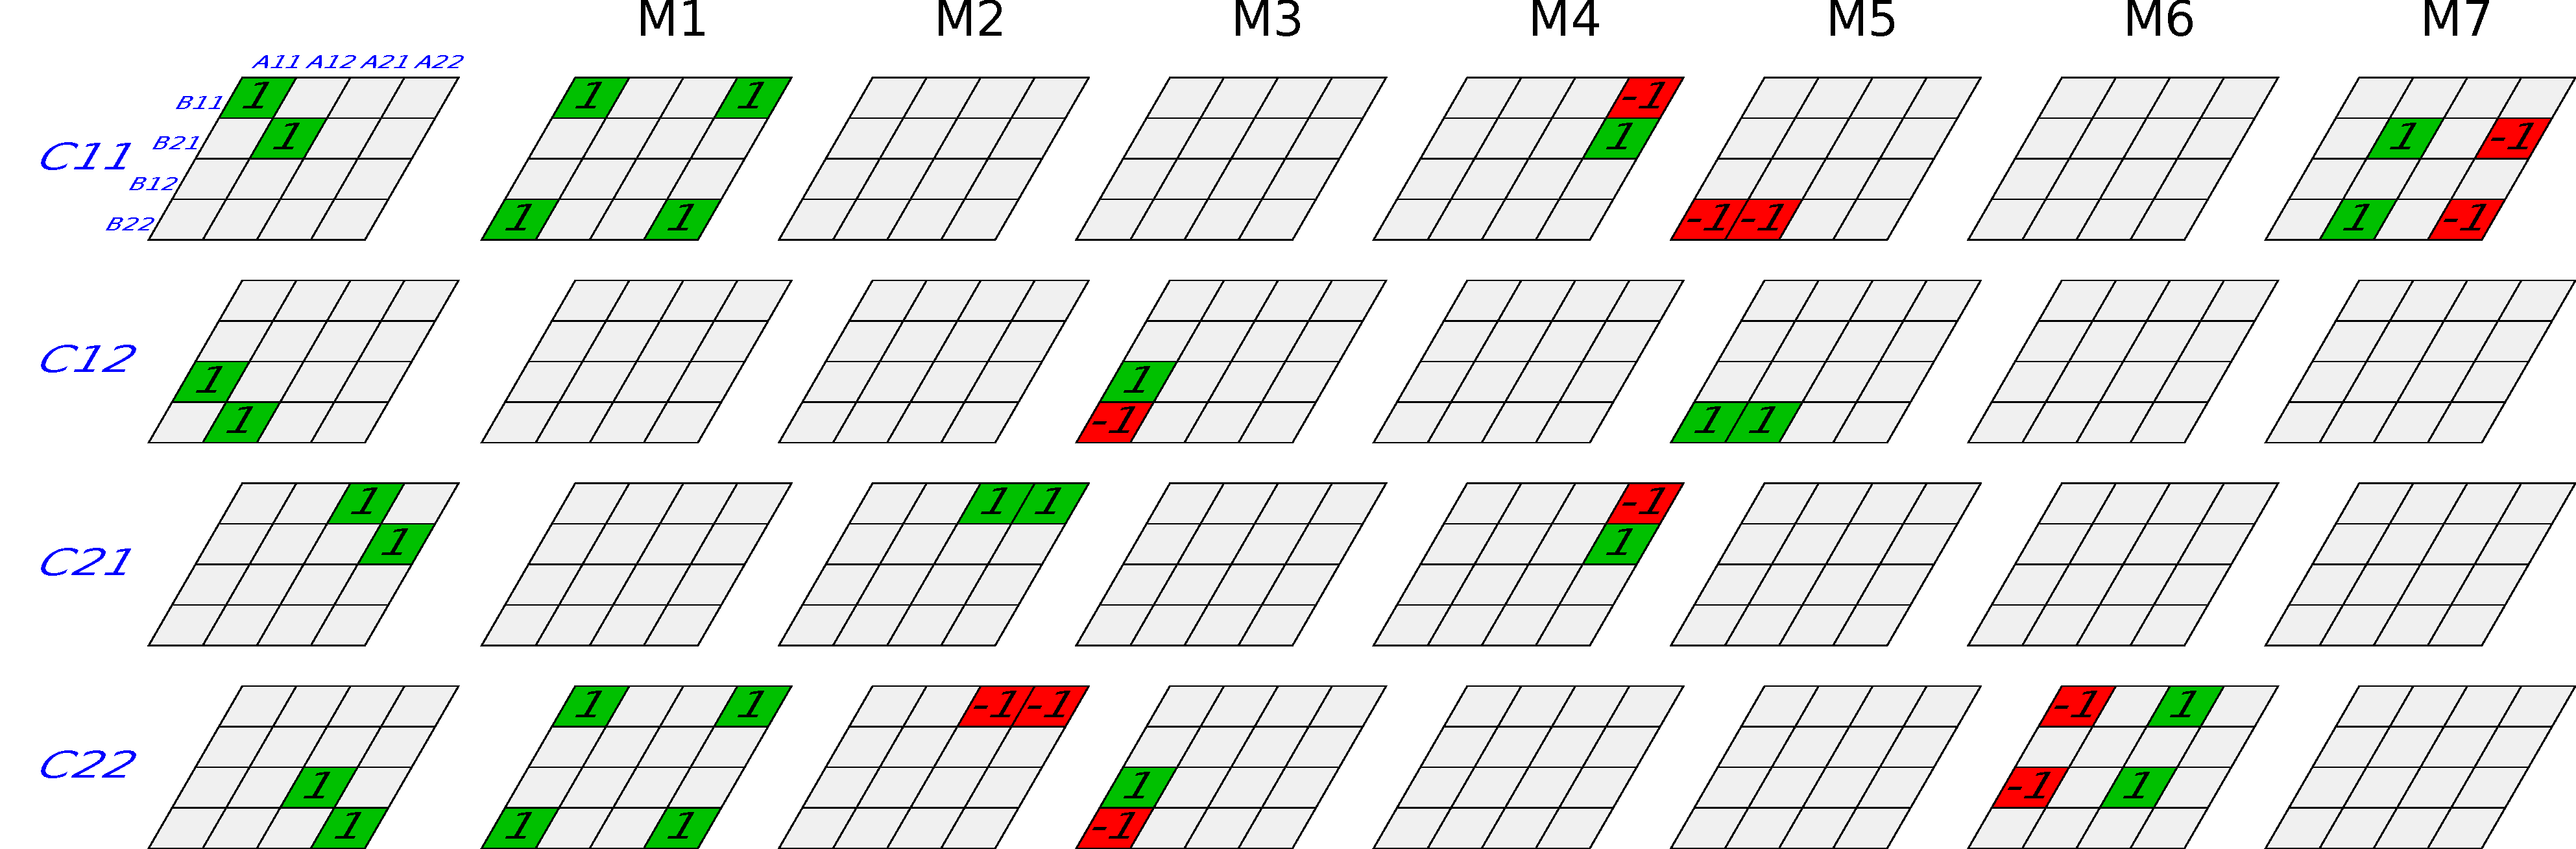
\includegraphics[width=\textwidth]{./images/strassen}
	\caption{Strassen (převzato z wikipedie, předělat?)}
	\label{fig:StrVis}
\end{figure}

Zápis Strassenova algoritmu vypadá následnovně:	

\begin{align}
A \cdot B = \begin{pmatrix}
 A_{1,1} & A_{1,2} \\
 A_{2,1} & A_{2,2} \\
\end{pmatrix} \cdot \begin{pmatrix}
 B_{1,1} & B_{1,2} \\
 B_{2,1} & B_{2,2} \\
\end{pmatrix} \\
M_{1} = (A_{1,1} + A_{2,2}) \cdot (B_{1,1} + B_{2,2}) \\
M_{2} = (A_{2,1} + A_{2,2}) \cdot B_{1,1} \\
M_{3} = A_{1,1} \cdot (B_{1,2} - B_{2,2}) \\
M_{4} = A_{2,2} \cdot (B_{2,1} - B_{1,1}) \\
M_{5} = (A_{1,1} + A_{1,2}) \cdot B_{2,2} \\
M_{6} = (A_{2,1} - A_{1,1}) \cdot (B_{1,1} + B_{1,2}) \\
M_{7} = (A_{1,2} - A_{2,2}) \cdot (B_{2,1} + B_{2,2}) \\
C = \begin{pmatrix}
 M_{1} + M_{4} - M_{5} + M_{7} & M_{3} + M_{5} \\
 M_{2} + M_{4} & M_{1} - M_{2} + M_{3} + M_{6}
\end{pmatrix}
\end{align}

V pseudokódu používáme procedury \texttt{offset-add} respektive \texttt{offset-sub}. Slouží ke sčítání respektive odečítání matic bloku prvků od nějakého offsetu y a x. Paremetry obou funkcí jsou: \texttt{offset-*}$(A,B,C,ay,ax,by,bx,cy,cx,n)$. 

\begin{algorithm}[H]
	\caption{Strassenův algoritmus}\label{mmm-strassen}
	\begin{algorithmic}[1]
		\Procedure{MMM-strassen}{$A,B,C,ay,ax,by,bx,cy,cx,n$}
		\If{$n = 1$}
			\State \texttt{$C[cy][cx]\gets C[cy][cx] + A[ay][ax] \cdot B[by][bx];$}
			\State \texttt{$return;$}
		\EndIf
  		\State \texttt{$h \gets n/2;$} \Comment{čtvrtina}
  		\State \texttt{$m[9] \gets initMatrices(9, h);$} \Comment{devět pomocných matic}
 % 	
	\State \texttt{offset-add$(a, a, m[8], ay, ax, ay + h, ax + h, 0, 0, h);$} \Comment{M1}
	\State \texttt{offset-add$(b, b, m[9], by, bx, by + h, bx + h, 0, 0, h);$}
	\State \texttt{MMM-strassen$(m[8], m[9], m[1], 0, 0, 0, 0, 0, 0, h);$}
%	
	\State \texttt{offset-add$(a, a, m[8], ay + h, ax, ay + h, ax + h, 0, 0, h);$} \Comment{M2}
	\State \texttt{MMM-strassen$(m[8], b, m[2], 0, 0, bx, by, 0, 0, h);$}
%	
	\State \texttt{offset-sub$(b, b, m[8], by, bx + h, by + h, bx + h, 0, 0, h);$} \Comment{M3}
	\State \texttt{MMM-strassen$(a, m[8], m[3], ay, ax, 0, 0, 0, 0, h);$}
%	
	\State \texttt{offset-sub$(b, b, m[8], by + h, bx, by, bx, 0, 0, h);$} \Comment{M4}
	\State \texttt{MMM-strassen$(a, m[8], m[4], ay + h, ax + h, 0, 0, 0, 0, h);$}
%	
	\State \texttt{offset-add$(a, a, m[8], ay, ax, ay, ax + h, 0, 0, h);$} \Comment{M5}
	\State \texttt{MMM-strassen$(m[8], b, m[5], 0, 0, by + h, bx + h, 0, 0, h);$}
%	
	\State \texttt{offset-sub$(a, a, m[8], ay + h, ax, ay, ax, 0, 0, h);$} \Comment{M6}
	\State \texttt{offset-add$(b, b, m[9], by, bx, by, bx + h, 0, 0, h);$}
	\State \texttt{MMM-strassen$(m[8], m[9], m[6], 0, 0, 0, 0, 0, 0, h);$}
%	
	\State \texttt{offset-sub$(a, a, m[8], ay, ax + h, ay + h, ax + h, 0, 0, h);$} \Comment{M7}
	\State \texttt{offset-add$(b, b, m[9], by + h, bx, by + h, bx + h, 0, 0, h);$}
	\State \texttt{MMM-strassen$(m[8], m[9], m[7], 0, 0, 0, 0, 0, 0, h);$}
%	
	\State \texttt{offset-add$(m[1], m[4], m[8], 0, 0, 0, 0, 0, 0, h);$} \Comment{c1,1}
	\State \texttt{offset-sub$(m[8], m[5], m[8], 0, 0, 0, 0, 0, 0, h);$}
	\State \texttt{offset-add$(m[8], m[7], c, 0, 0, 0, 0, cy, cx, h);$}
%	
	\State \texttt{offset-add$(m[3], m[5], c, 0, 0, 0, 0, cy, cx + h, h);$} \Comment{c1,2}
%	
	\State \texttt{offset-add$(m[2], m[4], c, 0, 0, 0, 0, cy + h, cx, h);$} \Comment{c2,1}
%	
	\State \texttt{offset-sub$(m[1], m[2], m[8], 0, 0, 0, 0, 0, 0, h);$} \Comment{c2,2}
	\State \texttt{offset-add$(m[8], m[3], m[8], 0, 0, 0, 0, 0, 0, h);$}
	\State \texttt{offset-add$(m[8], m[6], c, 0, 0, 0, 0, cy + h, cx + h, h);$}		
		\EndProcedure
	\end{algorithmic}
\end{algorithm}


Výpočet asymptotické složitosti vypočteme podobně jako u \texttt{MMM-recursive}, tedy mistrovskou metodou. 

TODO: mistrovska metoda

Stejně jako v předešlém algorimu, i zde demonstrujeme výpočet levého horního prvku matice z násobení dvou matic o velikosti dva. Místo parametrické matice použijeme desetinná čísla, abysme ukázali numerickou stabilitu Strassenova algoritmu. Pro ukázku budeme uvažovat počítač, který u čísel ukládá pouze pět cifer, znaménko a desetinnou čárku.	

Pomocí algoritmu podle definice, by takový počítač vypočítal součin dvou matic následnovně:

\begin{align}
\begin{pmatrix}
 30.234 & 0.5678 \\
 0.9123 & 10.456
\end{pmatrix} \cdot \begin{pmatrix}
 0.8912 & 0.3456 \\
 0.7891 & 9.999 \\
\end{pmatrix} = \begin{pmatrix}
 27.392 & \hdots \\
 \hdots & \hdots
\end{pmatrix}
\end{align}

Správný výsledek je $30.234 \times 0.8912 + 0.5678 \times 0.7891 = 26.9445408 + 0.44805098 = 27.39259178$.

Nyní výpočet provedeme pomocí Strassenova algoritmu:

\begin{align}
\begin{pmatrix}
 30.234 & 0.5678 \\
 0.9123 & 10.456
\end{pmatrix} \cdot \begin{pmatrix}
 0.8912 & 0.3456 \\
 0.7891 & 9.999
\end{pmatrix} \\
M_{1} = (30.234 + 10.456) \cdot (0.8912 + 9.999) = 443.12  \\
\hdots \\
M_{4} = 10.456 \cdot (0.7891 - 0.8912) = -1.067 \\
M_{5} = (30.234 + 0.5678) \cdot 9.999 = 307.98 \\
\hdots \\
M_{7} = (0.5678 - 10.456) \cdot (0.7891 + 9.999) = -106.67 \\
 \begin{pmatrix}
 M_{1} + M_{4} - M_{5} + M_{7} & \hdots \\
 \hdots & \hdots
\end{pmatrix} = \begin{pmatrix}
 27.403 & \hdots \\
 \hdots & \hdots
\end{pmatrix}
\end{align}

% zdroj http://math.nist.gov/MatrixMarket/data/Harwell-Boeing/oilgen/orsirr_1.html

Pro reálnou představu stability Strassenova algoritmu jsme provedli experiment, ve kterém jsme vynásobili dvě stejné matice (matice orsirr\_1, oriznuta na 1024x1024) algoritmem podle definice a Strassenovým algoritmem s různýmy práhy a sečetli všechny rozdíly mezi výsledky. Násobení probíhalo ve dvojté desetinné přesenosti, tedy v datovém typu \texttt{double} jazyka C99. Z grafu je vidět exponencionální růst chyby.

\begin{figure}[H]\centering
	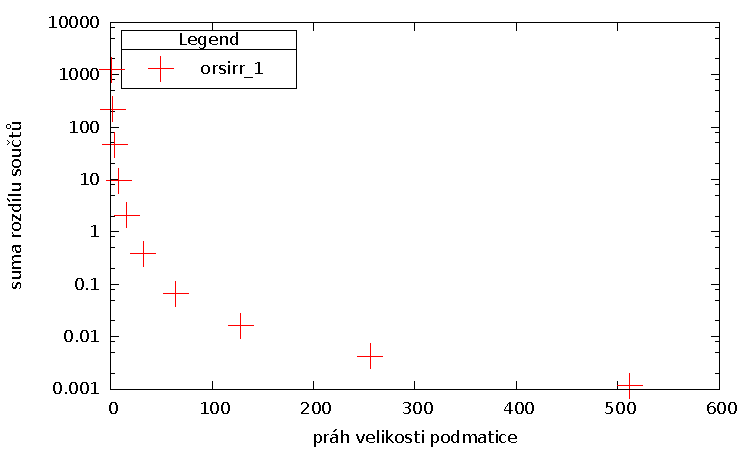
\includegraphics[width=\textwidth]{./images/strassen_stability}
	\caption{Strassen stability}
	\label{fig:Ukázka numerické stability Strassenova algoritmu}
\end{figure}

Strassenův algorimus lze ještě vylepšit. Algoritmům na stejném principu se říká Strassen-like. Pro sedm operací násobení je monžné snížit počet sčítání a odečítání. Pro jednoduchost zde ovšem uvádíme originalní algoritmus.

\section{Coppersmith-Winograd algoritmus}

TODO: rict ze ma dobrou O(n2735477), ale velkou konstantu a je v praxi zatim nepouzitelny

\section{Další algoritmy}

Existuje mnoho dalších algoritmů násobení matic. Zmíníme algoritmy vyhledávající vzory v řídkých maticích, například diagonály, co násobí jednotlivé vzory mezi sebou. \textbf{?muzu rict, ze to delat nebudu?} V této práci se zabýváme pouze algoritmy a formáty uložení pro (odkaz do sekce s typama ridkych matic).


%-----------------------------------------------------------------------------
%-----------------------------------------------------------------------------
%-----------------------------------------------------------------------------

\chapter{Formáty uložení řídkých matic}

\section{COO - Coordinate list}

\section{CSR - Compressed sparse row}

\section{BSR - Block Sparse Row}

\section{Quadtree}

\section{?}

TODO: tady jsem chtel spocictat kdy  se vyplati mit ridkou matici, ale lepsi bude tabulka

Pokud například uložíme matici o rozměrech 100x100 v dvojté přestnosti, bude zabírat \texttt{M x N x sizeof(double) = 100 x 100 x 8 = 80000B = 80kB}. Pokud zvolíme řídký formát matice, kde ke každému elementu uložíme i jeho x a y souřadnici, tak do 80kB uložíme \texttt{80000 / (sizeof(int)+sizeof(int)+sizeof(double)) = 80000/16= 5000} elementů. Pokud matice obsahuje více jak 50  \% nulových elementů, vyplatí se nám ji uložit do řídkého formátu.

%-----------------------------------------------------------------------------

\chapter{Modifikace formátu quadtree}

je to samostatnej bod v zadani tak by to mohla byt cela chapter

TODO: popsat nevyhody quadtree a obrazkama ukazat jak to udelat lip

neco jako quadtree loop unrolling


\chapter{Analýza a návrh}

? bud to nechapu nebo tuhle chapter smazu

XXX: napsat o tom, jak jsem pouzil spoustu knihoven. napr libc nebo math.
napsat o tom, jak jsem chtel scipy sparse, ale chtel jsem to co nejjednodussi

\chapter{Realizace}

\section{MatrixMarket}

TODO: posat format matrixmarket, ve kterem budu vsechno delat

\section{Optimalizace}

TODO: rict ze budeme verit -O3, ale popsat transformaci cyklu a loop-unrolling

\section{? Design implementace}

TODO: popsat OOP v C, moje testy

\section{Měření}

TODO: popsat jak to budu měřit, tedy cas z omp a cachegrind/callgrind (mozna solaris)






%%%%%%%%%%%%%%%%%%%%%%%%%%%%%%%%%%%%%%%%%%%%%%%%%%%%%%%%%%%%%%%%%%%%%%%%%%%%%%
%%%%%%%%%%%%%%%%%%%%%%%%%%%%%%%%%%%%%%%%%%%%%%%%%%%%%%%%%%%%%%%%%%%%%%%%%%%%%%
%%%%%%%%%%%%%%%%%%%%%%%%%%%%%%%%%%%%%%%%%%%%%%%%%%%%%%%%%%%%%%%%%%%%%%%%%%%%%%
%%%%%%%%%%%%%%%%%%%%%%%%%%%%%%%%%%%%%%%%%%%%%%%%%%%%%%%%%%%%%%%%%%%%%%%%%%%%%%
%%%%%%%%%%%%%%%%%%%%%%%%%%%%%%%%%%%%%%%%%%%%%%%%%%%%%%%%%%%%%%%%%%%%%%%%%%%%%%
%%%%%%%%%%%%%%%%%%%%%%%%%%%%%%%%%%%%%%%%%%%%%%%%%%%%%%%%%%%%%%%%%%%%%%%%%% end
%%%%%%%%%%%%%%%%%%%%%%%%%%%%%%%%%%%%%%%%%%%%%%%%%%%%%%%%%%%%%%%%%%%%%%%%%%%%%%
%%%%%%%%%%%%%%%%%%%%%%%%%%%%%%%%%%%%%%%%%%%%%%%%%%%%%%%%%%%%%%%%%%%%%%%%%%%%%%
%%%%%%%%%%%%%%%%%%%%%%%%%%%%%%%%%%%%%%%%%%%%%%%%%%%%%%%%%%%%%%%%%%%%%%%%%%%%%%
%%%%%%%%%%%%%%%%%%%%%%%%%%%%%%%%%%%%%%%%%%%%%%%%%%%%%%%%%%%%%%%%%%%%%%%%%%%%%%
%%%%%%%%%%%%%%%%%%%%%%%%%%%%%%%%%%%%%%%%%%%%%%%%%%%%%%%%%%%%%%%%%%%%%%%%%%%%%%

%\chapter{Cíl práce}

%\chapter{Analýza a návrh}

%\chapter{Realizace}

\begin{conclusion}
	%sem napište závěr Vaší práce
\end{conclusion}

\bibliographystyle{csn690}
\bibliography{mybibliographyfile}

\appendix

\chapter{Seznam použitých zkratek}
% \printglossaries
\begin{description}
	\item[GUI] Graphical user interface
	\item[XML] Extensible markup language
\end{description}

\nopagebreak[4]
\nopagebreak[4]

% !nesro
\listoffigures

\nopagebreak[4]
\nopagebreak[4]

\listofalgorithms*
% !!nesro

\nopagebreak[4]
\nopagebreak[4]

% % % % % % % % % % % % % % % % % % % % % % % % % % % % 
% % Tuto kapitolu z výsledné práce ODSTRAŇTE.
% % % % % % % % % % % % % % % % % % % % % % % % % % % % 
% 
% \chapter{Návod k~použití této šablony}
% 
% Tento dokument slouží jako základ pro napsání závěrečné práce na Fakultě informačních technologií ČVUT v~Praze.
% 
% \section{Výběr základu}
% 
% Vyberte si šablonu podle druhu práce (bakalářská, diplomová), jazyka (čeština, angličtina) a kódování (ASCII, \mbox{UTF-8}, \mbox{ISO-8859-2} neboli latin2 a nebo \mbox{Windows-1250}). 
% 
% V~české variantě naleznete šablony v~souborech pojmenovaných ve formátu práce\_kódování.tex. Typ může být:
% \begin{description}
% 	\item[BP] bakalářská práce,
% 	\item[DP] diplomová (magisterská) práce.
% \end{description}
% Kódování, ve kterém chcete psát, může být:
% \begin{description}
% 	\item[UTF-8] kódování Unicode,
% 	\item[ISO-8859-2] latin2,
% 	\item[Windows-1250] znaková sada 1250 Windows.
% \end{description}
% V~případě nejistoty ohledně kódování doporučujeme následující postup:
% \begin{enumerate}
% 	\item Otevřete šablony pro kódování UTF-8 v~editoru prostého textu, který chcete pro psaní práce použít -- pokud můžete texty s~diakritikou normálně přečíst, použijte tuto šablonu.
% 	\item V~opačném případě postupujte dále podle toho, jaký operační systém používáte:
% 	\begin{itemize}
% 		\item v~případě Windows použijte šablonu pro kódování \mbox{Windows-1250},
% 		\item jinak zkuste použít šablonu pro kódování \mbox{ISO-8859-2}.
% 	\end{itemize}
% \end{enumerate}
% 
% 
% V~anglické variantě jsou šablony pojmenované podle typu práce, možnosti jsou:
% \begin{description}
% 	\item[bachelors] bakalářská práce,
% 	\item[masters] diplomová (magisterská) práce.
% \end{description}
% 
% \section{Použití šablony}
% 
% Šablona je určena pro zpracování systémem \LaTeXe{}. Text je možné psát v~textovém editoru jako prostý text, lze však také využít specializovaný editor pro \LaTeX{}, např. Kile.
% 
% Pro získání tisknutelného výstupu z~takto vytvořeného souboru použijte příkaz \verb|pdflatex|, kterému předáte cestu k~souboru jako parametr. Vhodný editor pro \LaTeX{} toto udělá za Vás. \verb|pdfcslatex| ani \verb|cslatex| \emph{nebudou} s~těmito šablonami fungovat.
% 
% Více informací o~použití systému \LaTeX{} najdete např. v~\cite{wikilatex}.
% 
% \subsection{Typografie}
% 
% Při psaní dodržujte typografické konvence zvoleného jazyka. České \uv{uvozovky} zapisujte použitím příkazu \verb|\uv|, kterému v~parametru předáte text, jenž má být v~uvozovkách. Anglické otevírací uvozovky se v~\LaTeX{}u zadávají jako dva zpětné apostrofy, uzavírací uvozovky jako dva apostrofy. Často chybně uváděný symbol "{} (palce) nemá s~uvozovkami nic společného.
% 
% Dále je třeba zabránit zalomení řádky mezi některými slovy, v~češtině např. za jednopísmennými předložkami a spojkami (vyjma \uv{a}). To docílíte vložením pružné nezalomitelné mezery -- znakem \texttt{\textasciitilde}. V~tomto případě to není třeba dělat ručně, lze použít program \verb|vlna|.
% 
% Více o~typografii viz \cite{kobltypo}.
% 
% \subsection{Obrázky}
% 
% Pro umožnění vkládání obrázků je vhodné použít balíček \verb|graphicx|, samotné vložení se provede příkazem \verb|\includegraphics|. Takto je možné vkládat obrázky ve formátu PDF, PNG a JPEG jestliže používáte pdf\LaTeX{} nebo ve formátu EPS jestliže používáte \LaTeX{}. Doporučujeme preferovat vektorové obrázky před rastrovými (vyjma fotografií).
% 
% \subsubsection{Získání vhodného formátu}
% 
% Pro získání vektorových formátů PDF nebo EPS z~jiných lze použít některý z~vektorových grafických editorů. Pro převod rastrového obrázku na vektorový lze použít rasterizaci, kterou mnohé editory zvládají (např. Inkscape). Pro konverze lze použít též nástroje pro dávkové zpracování běžně dodávané s~\LaTeX{}em, např. \verb|epstopdf|.
% 
% \subsubsection{Plovoucí prostředí}
% 
% Příkazem \verb|\includegraphics| lze obrázky vkládat přímo, doporučujeme však použít plovoucí prostředí, konkrétně \verb|figure|. Například obrázek \ref{fig:float} byl vložen tímto způsobem. Vůbec přitom nevadí, když je obrázek umístěn jinde, než bylo původně zamýšleno -- je tomu tak hlavně kvůli dodržení typografických konvencí. Namísto vynucování konkrétní pozice obrázku doporučujeme používat odkazování z~textu (dvojice příkazů \verb|\label| a \verb|\ref|).
% 
% \begin{figure}\centering
% 	
\includegraphics[width=0.5\textwidth, angle=30]{cvut-logo-bw}
% 	\caption[Příklad obrázku]{Ukázkový obrázek v~plovoucím prostředí}\label{fig:float}
% \end{figure}
% 
% \subsubsection{Verze obrázků}
% 
% % Gnuplot BW i barevně
% Může se hodit mít více verzí stejného obrázku, např. pro barevný či černobílý tisk a nebo pro prezentaci. S~pomocí některých nástrojů na generování grafiky je to snadné.
% 
% Máte-li například graf vytvořený v programu Gnuplot, můžete jeho černobílou variantu (viz obr. \ref{fig:gnuplot-bw}) vytvořit parametrem \verb|monochrome dashed| příkazu \verb|set term|. Barevnou variantu (viz obr. \ref{fig:gnuplot-col}) vhodnou na prezentace lze vytvořit parametrem \verb|colour solid|.
% 
% \begin{figure}\centering
% 	\includegraphics{gnuplot-bw}
% 	\caption{Černobílá varianta obrázku generovaného programem Gnuplot}\label{fig:gnuplot-bw}
% \end{figure}
% 
% \begin{figure}\centering
% 	\includegraphics{gnuplot-col}
% 	\caption{Barevná varianta obrázku generovaného programem Gnuplot}\label{fig:gnuplot-col}
% \end{figure}
% 
% 
% \subsection{Tabulky}
% 
% Tabulky lze zadávat různě, např. v~prostředí \verb|tabular|, avšak pro jejich vkládání platí to samé, co pro obrázky -- použijte plovoucí prostředí, v~tomto případě \verb|table|. Například tabulka \ref{tab:matematika} byla vložena tímto způsobem.
% 
% \begin{table}\centering
% 	\caption[Příklad tabulky]{Zadávání matematiky}\label{tab:matematika}
% 	\begin{tabular}{|l|l|c|c|}\hline
% 		Typ		& Prostředí		& \LaTeX{}ovská zkratka	& \TeX{}ovská zkratka	\tabularnewline \hline \hline
% 		Text		& \verb|math|		& \verb|\(...\)|	& \verb|$...$|		\tabularnewline \hline
% 		Displayed	& \verb|displaymath|	& \verb|\[...\]|	& \verb|$$...$$|	\tabularnewline \hline
% 	\end{tabular}
% \end{table}
% 
% % % % % % % % % % % % % % % % % % % % % % % % % % % % 

\chapter{Obsah přiloženého CD}

%upravte podle skutecnosti

\begin{figure}
	\dirtree{%
		.1 readme.txt\DTcomment{stručný popis obsahu CD}.
		.1 exe\DTcomment{adresář se spustitelnou formou implementace}.
		.1 src.
		.2 impl\DTcomment{zdrojové kódy implementace}.
		.2 thesis\DTcomment{zdrojová forma práce ve formátu \LaTeX{}}.
		.1 text\DTcomment{text práce}.
		.2 thesis.pdf\DTcomment{text práce ve formátu PDF}.
		.2 thesis.ps\DTcomment{text práce ve formátu PS}.
	}
\end{figure}

\end{document}
